\documentclass[]{auvsi_doc}
\setkeys{auvsi_doc.cls}{
	AUVSITitle={Airframe Componenet Placement},
	AUVSILogoPath={./../logo.pdf}
}

% include extra packages, if needed
\usepackage{tabularx}
\usepackage{booktabs}
\usepackage{longtable}

\begin{document}

	\begin{AUVSITitlePage}
		\begin{artifacttable}
			\entry{AF-014, 0.1, 03-01-19, SS Engineering, Tyler Critchfield, CHECKED BY}
			% additional \entry{} commands for extra rows in the revision table, if needed
		\end{artifacttable}
	\end{AUVSITitlePage}

	% document contents (see below for LaTex commands that make your life easier)
	\section{Introduction}
	To have a stable and aerodynamically efficient flight, it is vital that the airframe have a center of gravity (CG) at a specific location - specifically, one that is in front of the aerodynamic center (about 1/4 chord of the main wings). In our analysis of the airframe (see AF-011), we determined this location to be 6.2 cm in front of the leading edge of the wing. In this artifact, we present the locations of the major components of the system in order to achieve this desired CG of the entire aircraft. Figure \ref{fig:comps} shows the placement of our main components in the airframe to achieve the desired CG. Table \ref{table:comps-placement} lists the exact x-locations (measured from the nose of the aircraft) of each component. Only the x-location is listed because component placement primarily affects longitudinal stability (pitch). The y and z-locations are not critical for our application. Other minor components are not listed here for simplicity - they weigh less, so their exact locations are not as critical. In addition, their locations are primarily constrained by the placement of these major components (i.e. they need to be placed near the components they interface with), so it is not necessary to explicitly outline each location. 

	\begin{figure}[h!]
		\centering
		\label{fig:comps}
		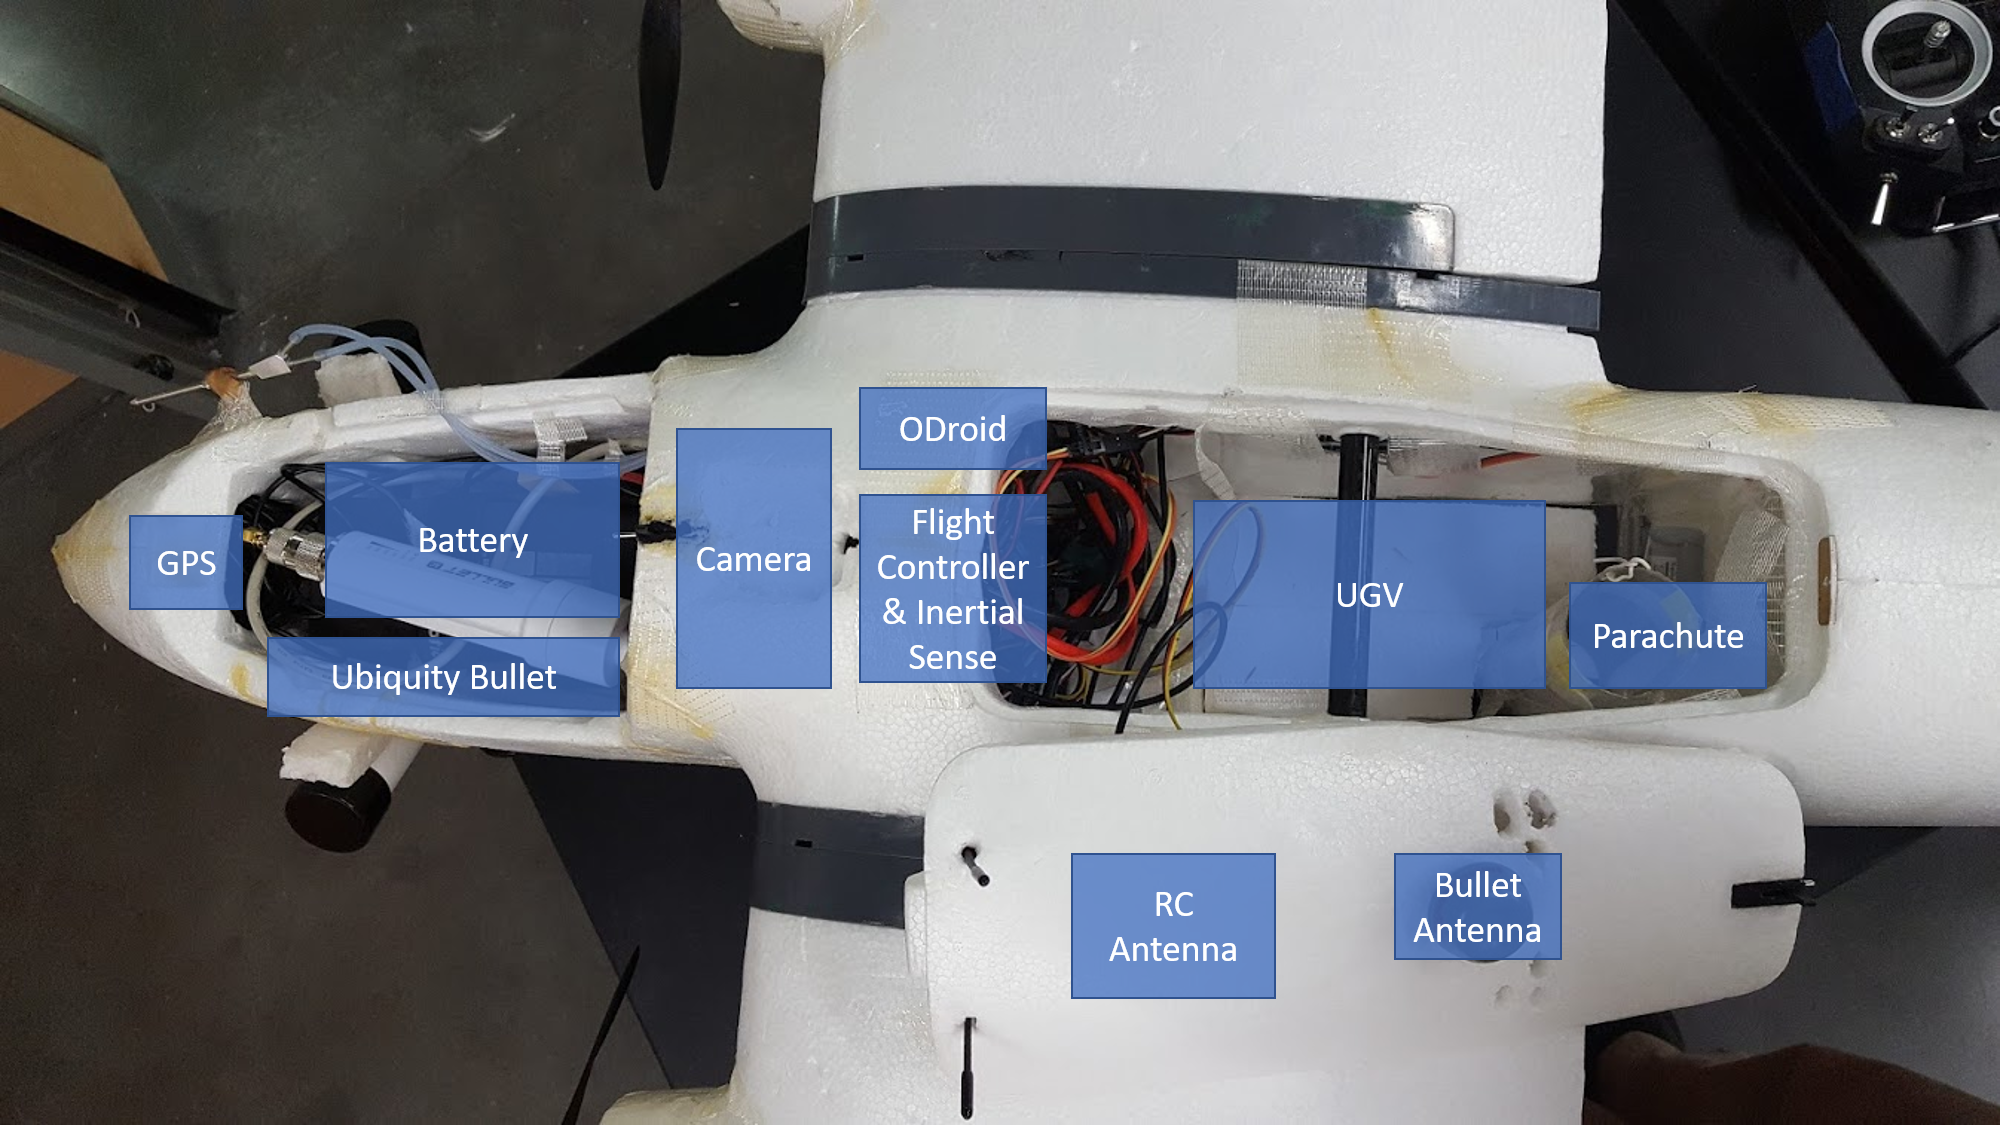
\includegraphics[width=.9\columnwidth]{comps}
		\caption{A top-down view of our airframe main compartment and location for each major component.}		
	\end{figure}

	%Begin table

	\begin{table}[h!]
		\begin{center}
			\caption{Exact location (measured from the nose of the plane) for each major component of the system.}
			\label{table:comps-placement}
			\begin{tabular}{c c c} 
				\toprule
				Index & CG x Location [cm] & Description \\
				\midrule
				1 & 21.5 & Battery \\
				2 & 17.5 & Ubiquity Bullet \\
				3 & 43.5 & Flight Controller/Inertial Sense \\
				4 & 63 & Bullet Antenna \\
				5 & 52.5 & RC Antenna \\
				6 & 68.5 & Parachute \\
				7 & 60.5 & UGV \\
				8 & 33.5 & Camera \\
				9 & 7.5 & GPS \\
				10 & 43.5 &ODroid \\
				\bottomrule
			\end{tabular}
		\end{center}
	\end{table}

\end{document}
